\documentclass[10pt,twocolumn]{article}
\usepackage[utf8]{inputenc}
\usepackage[spanish]{babel}
\usepackage{amsmath}
\usepackage{amsfonts}
\usepackage{amssymb}
\usepackage{graphicx}
\usepackage[left=2cm,right=2cm,top=2cm,bottom=2cm]{geometry}


\usepackage{listings}
\usepackage{color} %red, green, blue, yellow, cyan, magenta, black, white
\definecolor{mygreen}{RGB}{28,172,0} % color values Red, Green, Blue
\definecolor{mylilas}{RGB}{170,55,241}

\lstset{language=Matlab,% 
    %basicstyle=\color{red},
    breaklines=true,%
    morekeywords={matlab2tikz},
    keywordstyle=\color{blue},%
    morekeywords=[2]{1}, keywordstyle=[2]{\color{black}},
    identifierstyle=\color{black},%
    stringstyle=\color{mylilas},
    commentstyle=\color{mygreen},%
    showstringspaces=false,%without this there will be a symbol in the places where there is a space
    %numbers=left,%
    %numberstyle={\tiny \color{black}},% size of the numbers
    numbersep=9pt, % this defines how far the numbers are from the text
    emph=[1]{for,end,break},emphstyle=[1]\color{red}, %some words to emphasise
    %emph=[2]{word1,word2}, emphstyle=[2]{style},    
}

\author{Ivan Rene Ramirez Castro\\
            \small \textit{Pontificia Universidad Javeriana}\\
            \small \today}
\title{\textbf{Analisis de algoritmos para el software TicoBingo}}
\date{\vspace{-5ex}}

\begin{document}

\twocolumn[
  \begin{@twocolumnfalse}
    \maketitle
    \begin{abstract}
      \begin{center}
El presente trabajo aborda de una manera didáctica el análisis de algoritmos para el software TicoBingo, el cual es un juego de bingo en el que se pueden jugar hasta 10 cartones al mismo tiempo. El software es desarrollado en el lenguaje de programación Java, utilizando hilos para la ejecución de los cartones. El análisis de algoritmos se realiza mediante el calculo de la complejidad temporal y espacial de los algoritmos utilizados en el software. Se realiza una comparación entre los algoritmos utilizados en el software y una implementación de los mismos tratando de minimizar la complejidad temporal y espacial. Se concluye que la implementación de los algoritmos en el software TicoBingo es óptima, ya que en promedios de tiempo son muy similares a los algoritmos optimizados creados para este análisis.
      \end{center}
    \end{abstract}
    KEYWORDS: \textit{Algoritmos, Complejidad temporal, Complejidad espacial, Bingo, Java, Hilo\\ \\}
  \end{@twocolumnfalse}
  ]
 
 \section{Introducción}
 
 En el mundo de la informática, el análisis de algoritmos es una de las herramientas más importantes para el desarrollo de software. El análisis de algoritmos permite conocer la complejidad temporal y espacial de los algoritmos utilizados en un software, lo cual permite conocer la eficiencia de los mismos. El análisis de algoritmos se realiza mediante el cálculo de la complejidad temporal y espacial de los algoritmos utilizados en el software. La complejidad temporal de un algoritmo se define como el número de operaciones básicas que se realizan para resolver un problema. La complejidad espacial de un algoritmo se define como el número de variables que se utilizan para resolver un problema. 
 
 Para nuestro caso, el software TicoBingo tiene algurítmos que se ejecutan en un tiempo muy corto, algoritmos de validaciones de victoria, creacion de cartones, entre otros.

 Nuestro objetivo es realizar un análisis de estos algoritmos y compararlos con una implementación de los mismos tratando de minimizar la complejidad temporal y espacial.

\section{TicoBingo}
%   Cada cartón será 1 hilo separado que llenará su propio cartón y luego se duerme, 
% pero cuando se genera una bolita desde el programa principal (tómbola), se 
% despiertan todos los hilos al mismo tiempo para que busquen en su cartón si ese 
% número está presente y lo marcará (Colorea) en el cartón de la vista. Luego de 
% marcar la casilla con el número de la tómbola que acaba de salir, cada hilo debe 
% revisar si ha ganado la partida, y si gana, el juego termina y el jugador de ese cartón 
% gana, pero si no gana ningún cartón los hilos se duermen para esperar que salga otra 
% bolita de la tómbola.

El juego TicoBingo es un juego de bingo en el que se pueden jugar hasta 10 cartones al mismo tiempo. 
El software es desarrollado en el lenguaje de programación Java, utilizando hilos para la ejecución de los cartones.
El juego se inicia con la creación de los cartones, los cuales son creados de manera aleatoria teniendo en cuenta que no se repitan los números en un mismo cartón.
Cada cartón es un hilo separado que llenará su propio cartón y luego se duerme, pero cuando se genera una bolita desde el programa principal (tómbola), se despiertan todos los hilos al mismo tiempo para que busquen en su cartón si ese número está presente y lo marcará (Colorea) en el cartón de la vista. Luego de marcar la casilla con el número de la tómbola que acaba de salir, cada hilo debe revisar si ha ganado la partida, y si gana, el juego termina y el jugador de ese cartón gana, pero si no gana ningún cartón los hilos se duermen para esperar que salga otra bolita de la tómbola.


  \begin{figure}[h]
 	\centering
 	\includegraphics[width=0.5\textwidth]{ticobingointro.png}
 	\caption{Interfaz del juego TicoBingo}
 	\label{arreglo_pv}
 \end{figure}
 
El funcionamiento de una celda fotovoltaica se basa en el principio fundamental del efecto fotoeléctrico, el cuál, puede ser definido como un fenómeno en el que un electrón es expulsado de la banda conductora como resultado de la materia que absorbe la luz solar de una determinada longitud de onda. \cite{sreega2017design}.

\subsection{Modelo matemático}

La tarea principal del modelamiento consiste en producir una gráfica que represente el comportamiento de la corriente de salida y la potencia del SPVA, con respecto a la tensión en diferentes condiciones ambientales (temperatura e irradiación). \cite{shongwe2015comparative}.

El modelo del panel está basado en un circuito equivalente no ideal, que incluye las pérdidas dadas por las resistencias parásitas, conocido como el modelo de los cinco parámetros, donde la celda PV se modela como fuente de corriente y está conectada en paralelo al diodo que emula el fenómeno de polarización. Las resistencias $R_s$ y $R_{sh}$ están conectadas en serie y paralelo respectivamente. Este modelo es utilizado debido a su buena aproximación. \cite{vera2013maximum}.

El modelo planteado se representa a través del circuito que se muestra en la figura \ref{modelo_5parametros}, en donde se determina la siguiente ecuación partiendo de la Ley de Kirchhoff:

\begin{equation*}
I_{PV} = I_L - I_D - I_{R_{sh}}
\end{equation*}

  \begin{figure}[h]
 	\centering
 	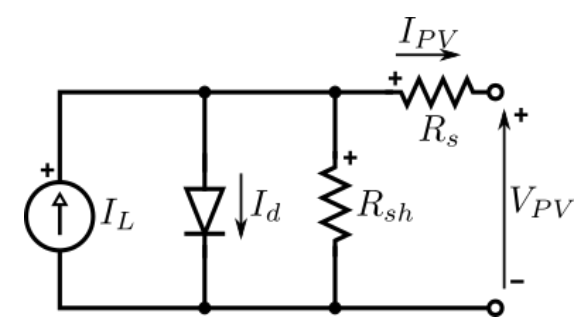
\includegraphics[width=0.4\textwidth]{modelo_5parametros.png}
 	\caption{Modelo de los cinco parámetros}
 	\label{modelo_5parametros}
 \end{figure}

Donde $I_L$ representa la fuente de corriente dada por la intensidad lumínica, $I_D$ es la corriente que pasa por el diodo y $I_{R_{sh}}$ corresponde a la corriente que pasa por la resistencia $R_{sh}$. \cite{riveracontrol}. Estas corrientes permiten representar el modelo del panel fotovoltaico de la siguiente manera:

\begin{multline}
I_{PV} = I_L - I_{sat} \left[ \exp \left( \dfrac{V_{pv} + I_{pv}R_s}{N_s a V_t} \right) - 1 \right] \\
- \dfrac{V_{pv} + I_{pv}R_s}{R_{sh}}
\end{multline}

\subsection{Panel Fotovoltaico Sunset PC-72}

El panel utilizado en el presente trabajo es el Sunset PC-72, el cuál cuenta con 72 celdas de silicio polycristalino. Se debe tener en cuenta la configuración de los paneles, bien sea en paralelo o en serie; es decir, si son ubicados en paralelo se eleva la corriente, y si son ubicados en serie se eleva el voltaje. En el cuadro \ref{datos_panel} se observan los datos proporcionados por el panel Sunset PC a condiciones estándar de prueba, a una temperatura de $25^{\circ}$C y una radiación de 1000 $\frac{W}{m^2}$.

\begin{table}[h]
    \begin{center}
   
        \begin{tabular}{ | c | c | }
           \hline $ P_{max} $ & 340 W \\ \hline
            $V_{oc} $ & 47.4 V \\ \hline
            $ V_{mpp}$ & 38.4 V \\ \hline
            $ I_{sc} $ & 9.35 A  \\ \hline
           $I_{mpp} $ & 8.84 A  \\ \hline
            $ N_{s} $ & 72  \\ \hline
            Coeficiente de temperatura  & 0.037 $\% /K$  \\ \hline
            Coeficiente de temperatura  & -0.32 $\% /K$  \\ \hline
            $ R_{s}$ & 0.39 $\Omega $  \\ \hline
             $R_{sh}$ & 545.82 $\Omega $  \\ \hline
\end{tabular}
\caption{Parámetros panel solar Sunset PX \cite{sunset}}
\label{datos_panel}
\end{center}
\end{table}

Dado que se requiere 4073 W de potencia, se diseña un arreglo de cuatro paneles en serie y tres en paralelo. Usando Simulink se pueden visualizar las curvas características del arreglo, ingresando los parámetros mencionados en el cuadro \ref{datos_panel}. En la figura \ref{curva_VI} y \ref{curva_PV} se observan las curvas para una temperatura de $25^{\circ}$C y diferentes valores de irradiancia ($\frac{W}{m^2}$).

\begin{figure}[h!]
    \centering
    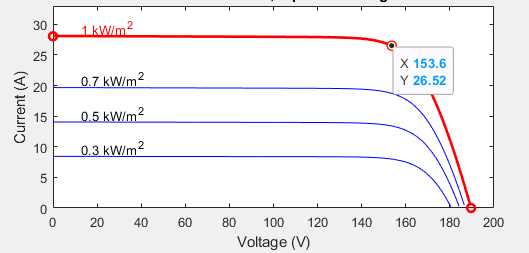
\includegraphics[width=0.5\textwidth]{VI_CURVA.png}
    \caption{Curva VI a una temperatura de $25^{\circ}$C}
    \label{curva_VI}
\end{figure}

\begin{figure}[h!]
    \centering
    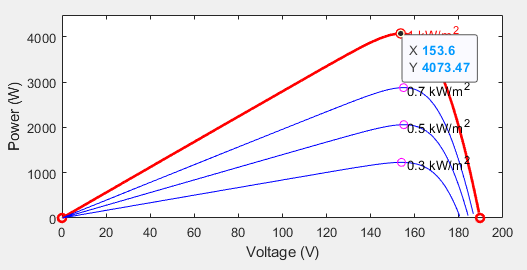
\includegraphics[width=0.5\textwidth]{PV_CURVA.png}
    \caption{Curva PV a una temperatura de $25^{\circ}$C}
    \label{curva_PV}
\end{figure}

\section{Modelamiento del convertidor boost}

Cuando se habla de un sistema fotovoltaico completo conectado a la red, se debe tener en cuenta diferentes etapas desde la producción de energía eléctrica en los paneles solares hasta la correcta entrega de la energía a la red como se muestra en la figura \ref{pv_system_full}. Para el presente trabajo, se centrará el estudio en el convertidor Boost.

\begin{figure}[h!]
    \centering
    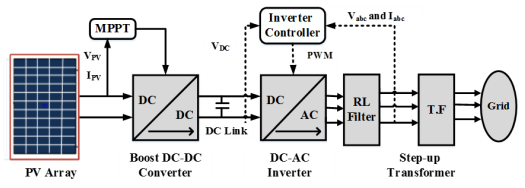
\includegraphics[width=0.5\textwidth]{pv_system_full.png}
    \caption{Diagrama simplificado de la red conectada del sistema fotovoltaico.}
    \label{pv_system_full}
\end{figure}

El circuito eléctrico de dicho convertidor se muestra en la figura \ref{circuito_boost}, y se conoce como elevador ya que la tensión de salida es mayor que la tensión de entrada. Está compuesta de un inductor elevado, un interruptor electrónico, un diodo, un filtro de salida capacitancia y la carga.\cite{pradipkumar2013design}.

 \begin{figure}[h]
	\centering
	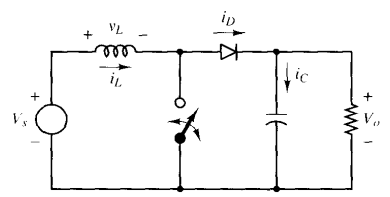
\includegraphics[width=0.4\textwidth]{circuito_boost.png}
	\caption{Circuito de un convertidor elevador}
	\label{circuito_boost}
\end{figure}

\subsection{Diseño del convertidor}

De acuerdo con \cite{mohan2009electronica} se desarrolla el diseño del convertidor siguiente las siguientes suposiciones para el primer ejemplo: 

\begin{enumerate}
	\item El circuito opera en régimen permanente.
	\item El periodo de conmutación es T y el interruptor está cerrado un tiempo DT.
	\item La corriente en la bobina es permanente.
	\item El condensador es muy grande y la tensión de salida se mantiene constante.
	\item Los componentes son ideales.
\end{enumerate}

Como primer ejemplo, el convertidor que se va a diseñar debe presentar una salida de 330 V a partir de una fuente de 153.6 V. Esta tensión de entrada es tomada en cuenta a partir de la tensión en el punto de máxima potencia de la figura \ref{curva_PV} a una irradiancia de 1000 $W/m^2$. La corriente en la bobina será permanente y el rizado de la tensión de salida debe ser menor que el 1 por ciento. La carga es una resistencia de 100 $\Omega$ y se supone que los componentes son ideales.

En primer lugar, se determina el ciclo de trabajo:

\begin{equation*}
	D = 1 - \frac{V_s}{V_o} = 1 - \frac{153.6}{330} = 0.5345
\end{equation*}

Si seleccionamos una frecuencia de conmutación de 25 kHz, superior al rango auditivo, podemos obtener la inductancia mínima para corriente permanente:

\begin{equation*}
	\begin{matrix}
		L_{min} = \frac{D\left ( 1- D \right )^2 R}{2f} = \frac{0.5345 \left ( 1 - 0.5345 \right )^2 100}{2\left ( 25000 \right )} \\
		= 231.64 \mu H
	\end{matrix}
\end{equation*}

Con el fin de mantener un margen para asegurar corriente permanente, definimos $L = 250 \mu H$. Se debe tener en cuenta que $L$ y $f$ se seleccionaron arbitrariamente, y que existen otras combinaciones que producirán corriente permanente.\\

Ahora:

\begin{equation*}
	I_L = \dfrac{V_s}{\left ( 1-D \right )^2 R} = \dfrac{153.6}{\left ( 1-0.5345 \right )^2\cdot 100} = 7.0885 \textup{A}
\end{equation*}

\begin{equation*}
	\dfrac{\Delta i_L}{2} = \dfrac{V_s DT}{2L} = \dfrac{\left ( 153.6 \right )\left ( 0.5345 \right )}{\left ( 2 \right )\left ( 250 \right )\left ( 10 \right )^{-6}\left ( 25000 \right )} = 6.5679 \textup{A}
\end{equation*}

\begin{equation*}
	I_{max} = 7.0885 + 6.5679 = 13.6564 \textup{A}
\end{equation*}

\begin{equation*}
	I_{min} = 7.0885  6.5679 = 0.5206 \textup{A}
\end{equation*}

Finalmente se calcula el rizado de la tensión de salida:

\begin{equation*}
	\begin{matrix}
		\cfrac{\Delta V_o}{v_o} = \cfrac{D}{RCf} < 1 \% \\ 
		C > \cfrac{D}{Rf\left ( \cfrac{\Delta V_o}{v_o} \right )} = \cfrac{0.5345}{\left ( 100 \right )\left ( 25 \right )\left ( 10 \right )^{3}\left ( 0.01 \right )} = 21.38 \mu \textup{F}
	\end{matrix}
\end{equation*}

\subsection{Simulación del convertidor elevador}

\subsubsection{Convertidor boost con tensión constante}

Partiendo de los datos obtenidos en la sección anterior, se procede a simular el comportamiento de la corriente y la tensión en los elementos que conforman el circuito usando Simulink como se muestra en la figura \ref{circuito_boost_lazoabierto}. Las formas de onda de la tensión y la corriente del convertidor elevador son mostradas en la figura \ref{curvas_lazoabierto}.

\begin{figure}[h]
	\centering
	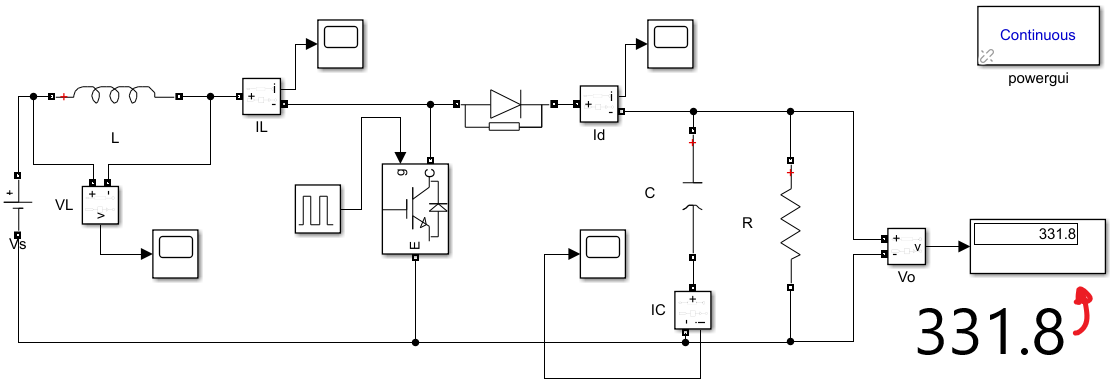
\includegraphics[width=0.5\textwidth]{circuito_Boost_lazoabierto.png}
	\caption{Esquema en simulink del circuito elevador en lazo abierto}
	\label{circuito_boost_lazoabierto}
\end{figure}

\begin{figure}[h]
	\centering
	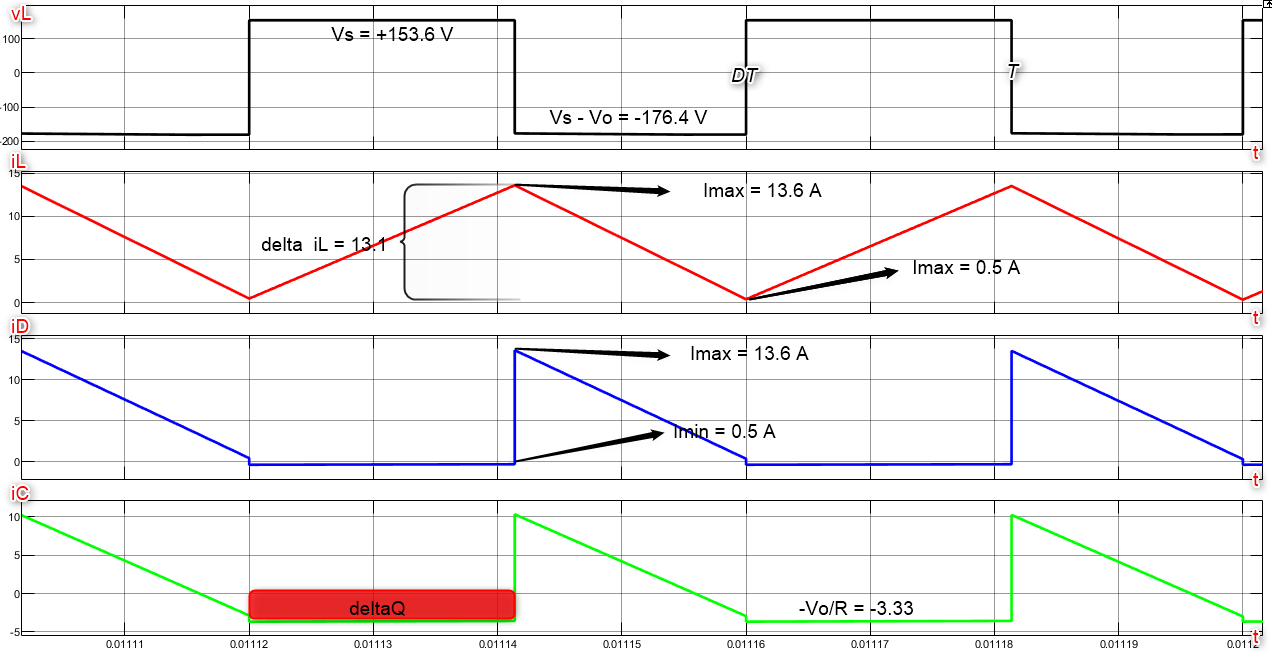
\includegraphics[width=0.5\textwidth]{curvas_lazoabierto.png}
	\caption{Formas de onda del convertidor elevador: Tensión en la bobina, corriente en la bobina, corriente en el diodo y corriente en el condensador.}
	\label{curvas_lazoabierto}
\end{figure}

\subsubsection{Convertidor boost con PV}

Una vez comprobado nuestro diseño a través de Simulink, ahora realizamos una modificación en la fuente de entrada. Esta vez se simula el comportamiento del circuito utilizando el arreglo fotovoltaico Sunset PC-72 como se observa en la figura \ref{circuito_boost_pv} con las especificaciones del cuadro \ref{datos_panel}. Para la simulación se toma como entrada una temperatura de $25^{\circ}$C y una radiación de 1000 $\frac{W}{m^2}$.
El comportamiento de las formas de onda mostradas en la figura \ref{curvas_lazoabierto} varían de acuerdo a la figura \ref{boost_pv}. Además en la figura \ref{boost2_pv} se observa el comportamiento de la tensión y corriente del arreglo PV y de la carga.



\begin{figure}[h!]
	\centering
	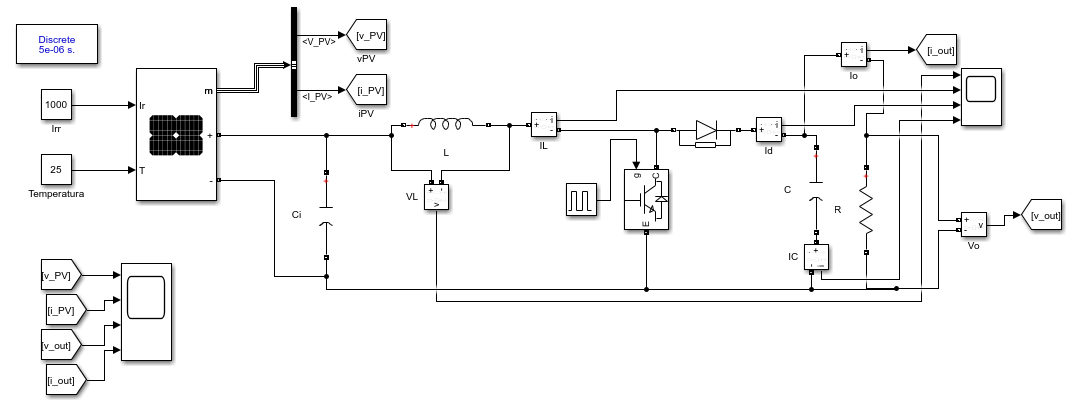
\includegraphics[width=0.5\textwidth]{circuito_Boost_lazoabierto_pv.png}
	\caption{Circuito del convertidor elevador utilizando un arreglo PV}
	\label{circuito_boost_pv}
\end{figure}

 \begin{figure}[h!]
	\centering
	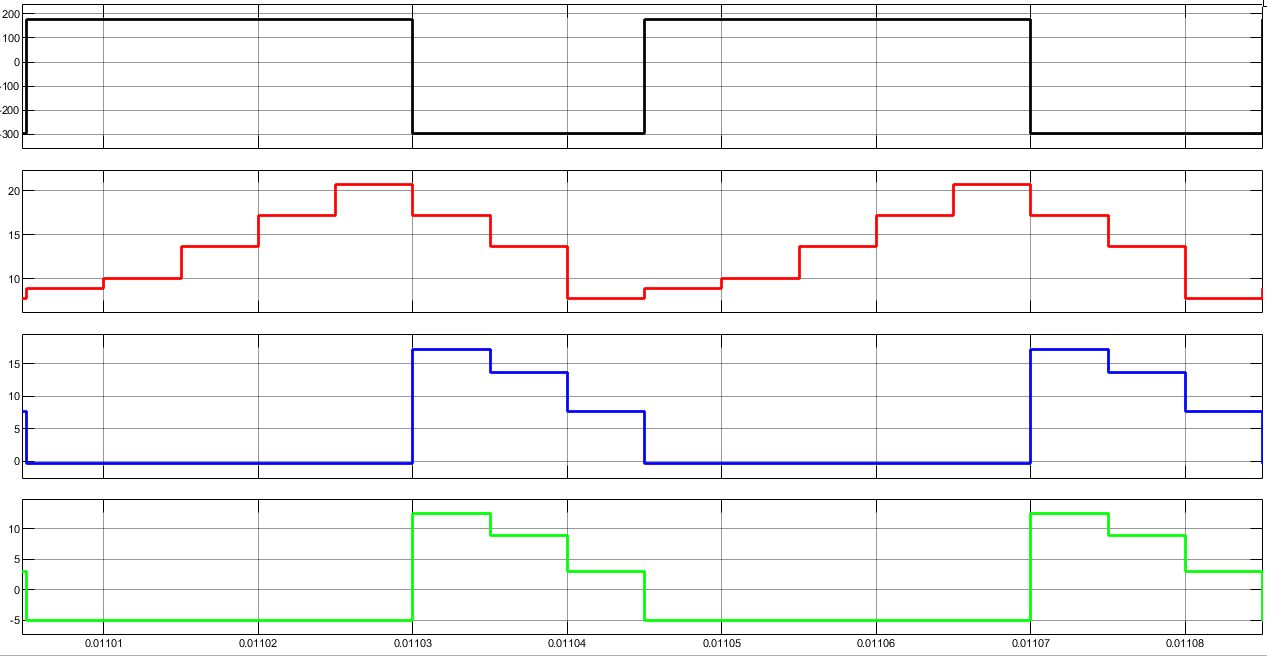
\includegraphics[width=0.5\textwidth]{curvas_lazoabierto_pv.png}
	\caption{Formas de onda del convertidor elevador: Tensión en la bobina, corriente en la bobina, corriente en el diodo y corriente en el condensador. Utilizando el arreglo PV Sunset PC-72}
	\label{boost_pv}
\end{figure}

\begin{figure}[h!]
	\centering
	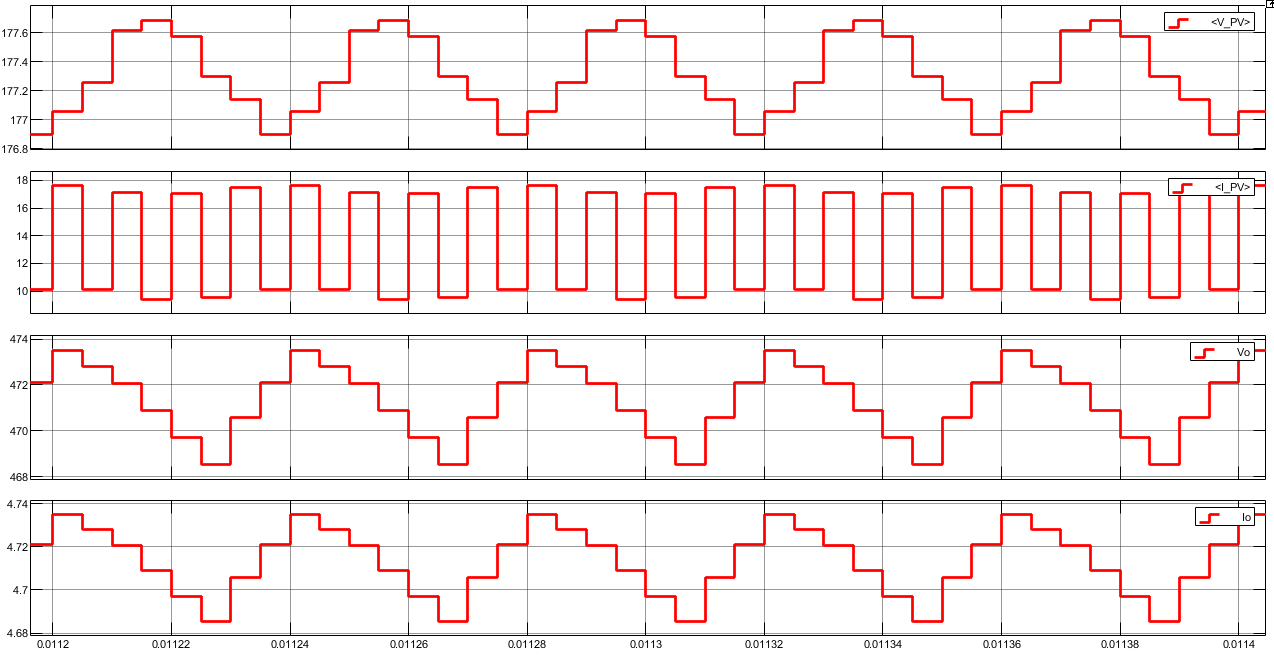
\includegraphics[width=0.5\textwidth]{curvas2_lazoabierto_pv.png}
	\caption{Formas de onda de la tensión PV, la corriente PV, la tensión en la carga y la corriente en la carga.}
	\label{boost2_pv}
\end{figure}

\section{Seguimiento del punto de máxima potencia}

Una de las tareas más importantes de los sistemas fotovoltaicos es extraer de forma confiable y rápida la máxima energía solar disponible en diversos escenarios ambientales. Esta tarea se conoce como seguimiento de máxima potencia (MPPT por sus siglas en inglés). \cite{motahhir2020most}.

Se sabe que la mayoría de los algoritmos de MPPT puden tener un rendimiento aceptable para sistemas fotovoltaicos que trabajen bajo irradiancia solar uniforme, no obstante el MPPT se vuelve complejo en condiciones de sombreado parcial, debido a que la tensión de salida del sistema se vuelve altamente no lineal en tales condiciones. \cite{yang2020comprehensive}.

Dentro de los algoritmos mas comunes para MPPT son: Perturb and Observe (P$\&$O), Hill climbing (HC), y incremental conductance (INC). Estos a menudo pueden tener un rendimiento decente en condiciones uniformes, ya que sólo hay un MPP que varía con la irradiancia solar o con la temperatura.

\subsection{Algoritmo MPPT basado en P$\&$O}

El algoritmo de optimización P$\&$O consiste en variar la tensión de referencia o la corriente de entrada del convertidor. Después, se mide la cantidad de potencia convertida desde el panel. Si es mayor que la potencia medida anteriormente, la referencia de tensión se incrementa constantemente en la misma proporción, y si no se disminuye. Estos pasos se toman continuamente para encontrar el MPPT óptimo. \cite{tobon2017maximum}.

La tensión en los terminales del sistema fotovoltaico se ve perturbada en cada ciclo del MPPT a intervalos de muestreo $T_S$, por lo que un vez alcanzado el punto de máxima potencia, el algoritmo P$\&$O oscilará alrededor de este punto resultando una pérdida de potencia del sistema PV, especialmente donde las condiciones atmosféricas varíen lentamente. En la figura \ref{po_algor} se puede observar el diagrama de flujo del algoritmo P$\&$O. \cite{molina2007analisis}

La figura \ref{po_operacion} muestra la potencia de salida PV con resspecto a la tensión de la carga para una radiación específica. Como se puede observar, existen dos ubicaciones para movilizarse de un punto A ( $\frac{dP}{dV} > 0$) hacia un punto B ($\frac{dP}{dV} < 0$). Cuando se utiliza un tamaño de
paso pequeño de la tensión, se alcanzará oscilaciones de estado estacionario con un resultado de respuesta MPPT
lenta. \cite{abdelwahab2020comparative}.

En la figura \ref{MPPT} se puede observar el esquema de funcionamiento del método de seguimiento del punto de máxima potencia para nuestro circuito (En el esquema se representan elementos ideales).

 \begin{figure}[h!]
	\centering
	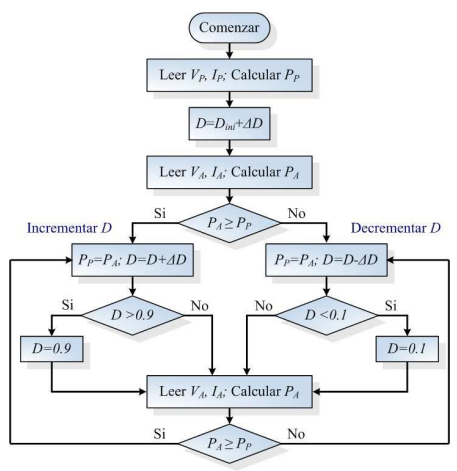
\includegraphics[width=0.5\textwidth]{po_algor.png}
	\caption{Diagrama de flujo del algoritmo P$\&$O \cite{molina2007analisis}.}
	\label{po_algor}
\end{figure}

 \begin{figure}[h!]
	\centering
	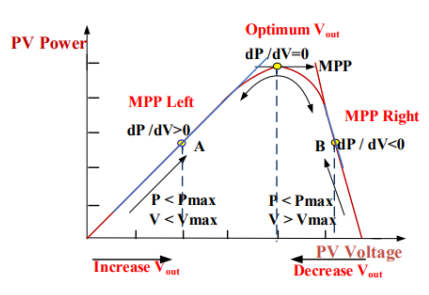
\includegraphics[width=0.5\textwidth]{po_operacion.png}
	\caption{Modo de operación algoritmo P$\&$O.}
	\label{po_operacion}
\end{figure}

 \begin{figure}[h!]
	\centering
	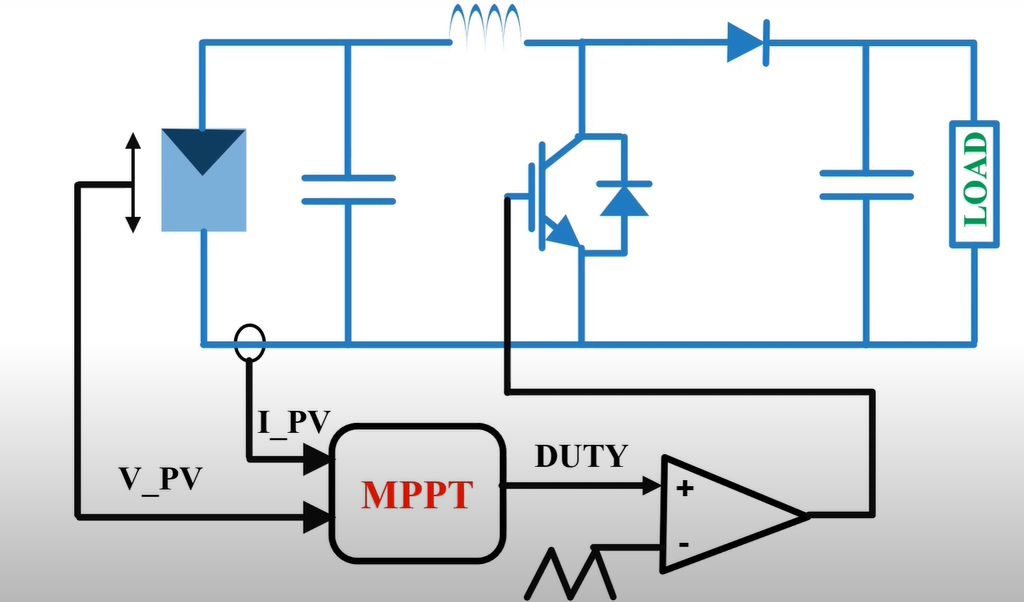
\includegraphics[width=0.35\textwidth]{mppt_DUTY.png}
	\caption{Implementación MPPT}
	\label{MPPT}
\end{figure}


\subsection{Programación del algoritmo P$\&$O}

A continuación se muestra un script que se implementará como una función del algoritmo P$\&$O para Simulink.

\begin{lstlisting} 
	function duty = MPPT_algorithm(vpv, ipv, delta)
	
	duty_init = 0.1;
	% min and max value are used to limit duty between 0 and 0.85
	duty_min = 0;
	duty_max = 0.85;
	
	persistent Vold Pold duty_old;
	% persistent variable type can be store the data
	% we need the old data by obtain difference between
	% old and new value
	if isempty(Vold)
	Vold = 0;
	Pold = 0;
	duty_old = duty_init;
	end
	P = vpv*ipv; % power
	dV = vpv - Vold; % difference between old and new value
	dP = P - Pold; % difference between old and new power
	
	
	% The algorithm is below search the dP/dV=0
	% if the derivative equal to zero
	% duty will not change
	% if old and new power not equal
	% &
	% pv_voltage bigger than 30V
	% the algorithm will works
	if dP ~= 0 && vpv > 30
	if dP < 0
	if dV < 0
	duty = duty_old - delta;
	else
	duty = duty_old + delta;
	end
	else
	if dV < 0
	duty = duty_old + delta;
	else
	duty = duty_old - delta;
	end
	end
	else
	duty = duty_old
	end
	
	% the below if will limits the duty between min and max
	if duty >= duty_max
	duty = duty_max;
	elseif duty < duty_min
	duty = duty_min;
	end
	
	% stored data
	duty_old = duty;
	Vold = vpv;
	Pold = P;
\end{lstlisting}

\section{Resultados de la simulación y discusión}

La representación como fuente de voltaje del capacitor de carga interactuando con un inversor conectado a la red, es el modelo más común para conexiones de dc con un inversor a lazo cerrado, considerando resistencias parásitas en los elementos pasivos del convertidor dc/dc y en el capacitor de carga, el esquema eléctrico usado se presenta en la figura \ref{circuitoboost_completo}.

 \begin{figure}[h]
	\centering
	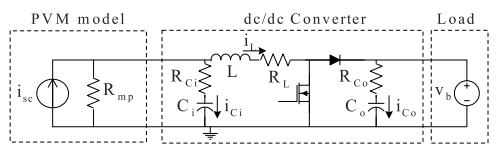
\includegraphics[width=0.5\textwidth]{boost_parasito.png}
	\caption{Modelo considerando pérdidas parásitas y fuente de voltaje como capacitor de carga.}
	\label{circuitoboost_completo}
\end{figure}

Como se mencionó anteriormente, en la figura \ref{curva_PV} se puede observar que existen puntos en los cuáles las gráficas de potencia alcanzan un valor máximo denominado MPP, allí se garantiza que para estos valores de potencia el módulo fotovoltaico esté entregando la máxima potencia disponible, y su posición varía dependiendo de las condiciones de irradianza y temperatura.

Para nuestro modelo más realista, introduciremos en la entrada diferentes valores de irradiancia en diferentes lapsos de tiempo de 0.25 segundos de la siguiente manera: [0, 0, 300, 300, 500, 700, 1000, 1000, 500, 500, 0, 0]. En la figura \ref{converter1} tenemos la simulación del circuito en donde la máxima potencia es de 4073.47 W a una temperatura de $25^{\circ}$C y una radiación de 1000 $\frac{W}{m^2}$.

 \begin{figure}[h!]
	\centering
	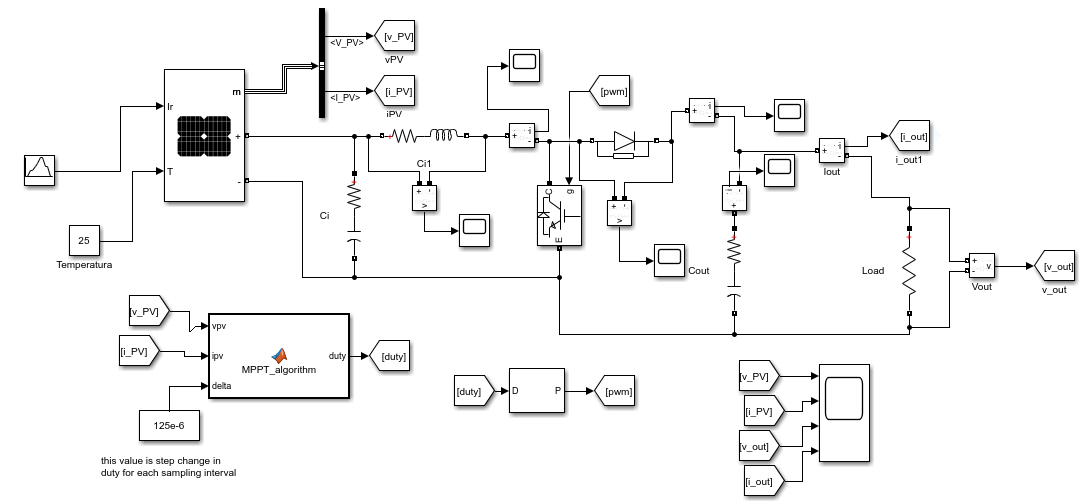
\includegraphics[width=0.5\textwidth]{converter2.png}
	\caption{ Convertidor boost sin MPPT}
	\label{converter1}
\end{figure}

Ahora, necesitamos una señal de ciclo de trabajo para determinar la relación de éste con la de PWM. Debido a que queremos controlar la potencia dependiendo del punto de potencia máxima, que a su vez depende de la irradiación.

El algoritmo MPPT determina los MPPs por la búsqueda de la derivada $ \frac{dP}{dV}  = 0$. En la figura \ref{converter2} se muestra el modelo con la función MPPT algorithm incluida. Y en la figura \ref{curvas1} se puede observar el comportamiento de la corriente y la tensión del panel y de la carga.

 \begin{figure}[h!]
	\centering
	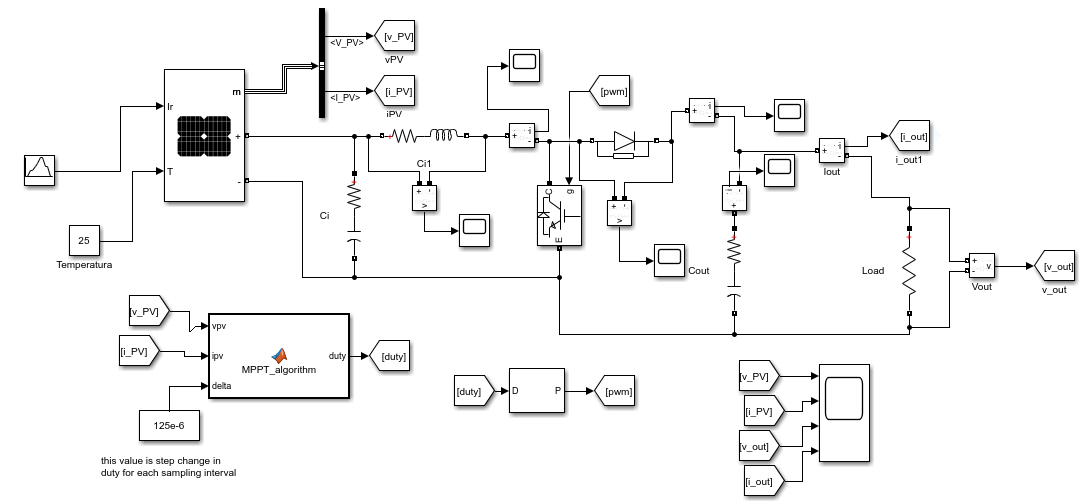
\includegraphics[width=0.5\textwidth]{converter2.png}
	\caption{Convertidor boost con MPPT}
	\label{converter2}
\end{figure}

 \begin{figure}[h!]
	\centering
	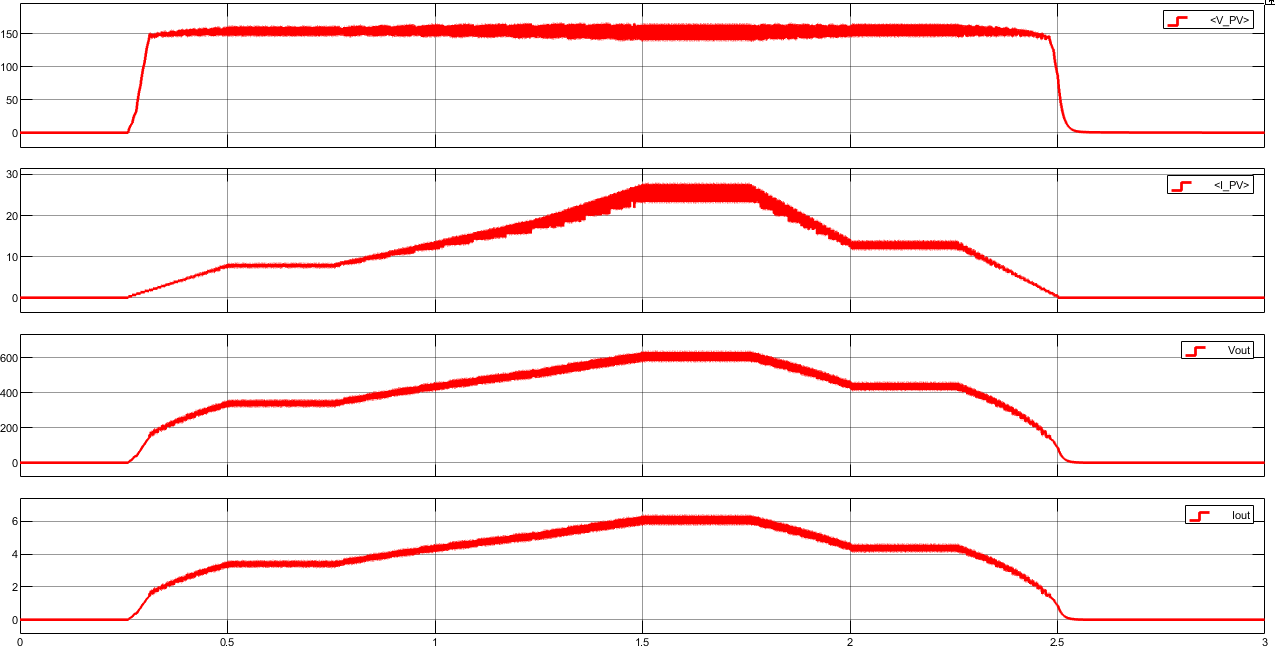
\includegraphics[width=0.5\textwidth]{curvas1.png}
	\caption{Comportamiento de $V_{PV}$, $I_{PV}$, $V_o$, $I_o$}
	\label{curvas1}
\end{figure}

Ahora podemos evaluar el comportamiento de la potencia. Para ello necesitamos una curva de potencia ideal para calcular la eficiencia del algoritmo MPPT. En la figura \ref{potencia} se observan los bloques usados en simulink. Y en la figura \ref{potencia_curvas} se muestra la comparación de las curvas de potencia del PV.

\begin{figure}[h!]
	\centering
	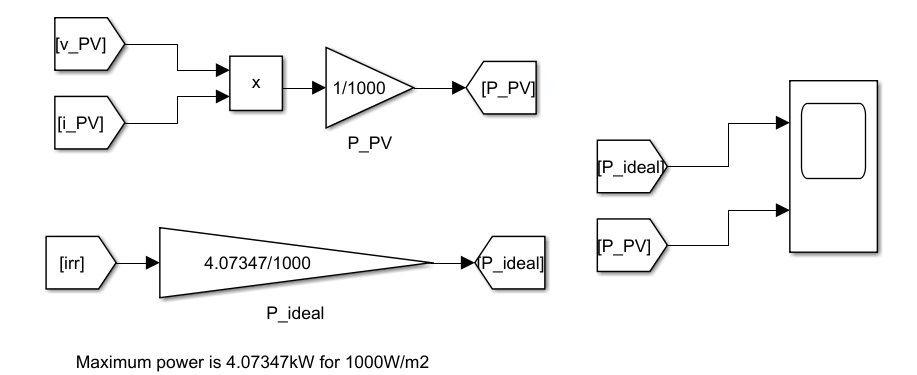
\includegraphics[width=0.5\textwidth]{potencia.png}
	\caption{Bloques para la comparación de la potencia real con la potencia ideal del PV}
	\label{potencia}
\end{figure}

\begin{figure}[h!]
	\centering
	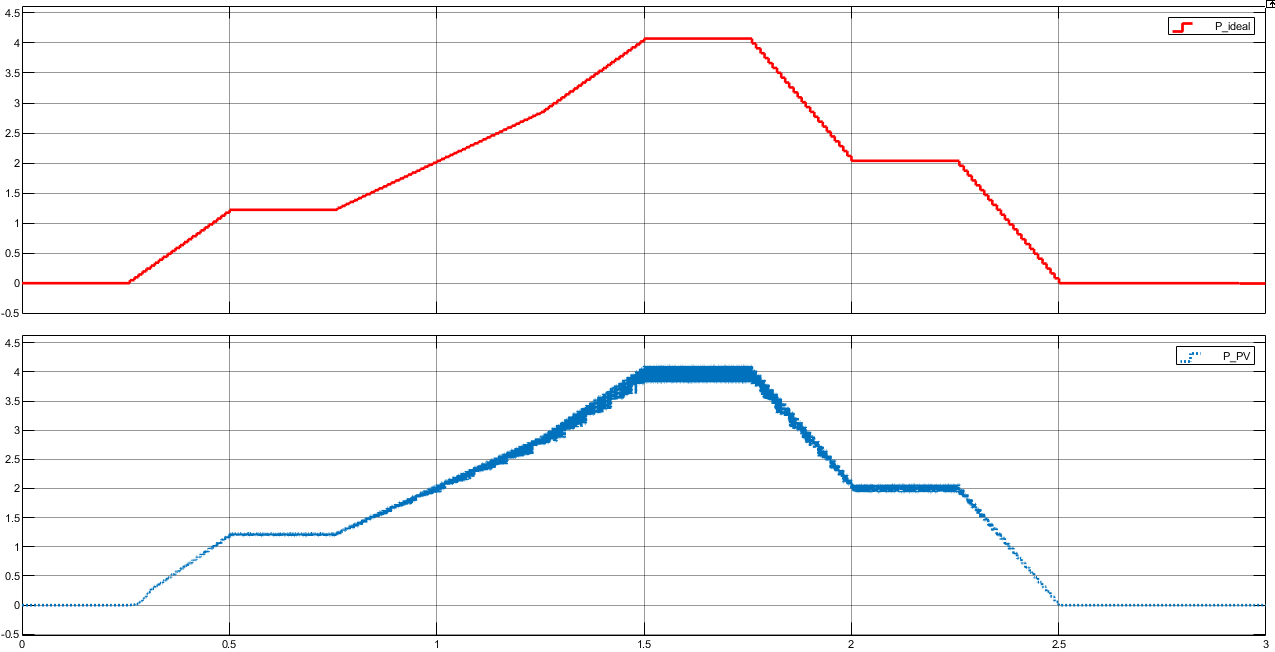
\includegraphics[width=0.5\textwidth]{potencia_curvas.png}
	\caption{Comparación de la potencia real con la potencia ideal del PV}
	\label{potencia_curvas}
\end{figure}

Con estos resultados se puede calcular la eficiencia del modelo obteniéndose el resultado mostrado en la figura \ref{eficiencia}. La eficiencia se ve aproximadamente mayor a 0.96.

\begin{figure}[h!]
	\centering
	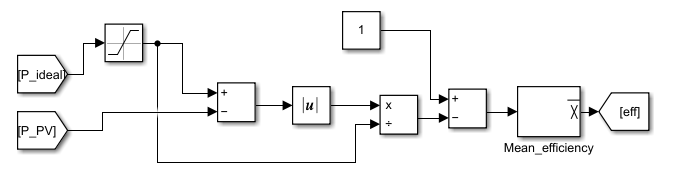
\includegraphics[width=0.5\textwidth]{eficiencia2.png}
	\caption{Bloque para calcular la eficiencia media de la potencia del modelo propuesto}
	\label{eficiencia}
\end{figure}

\begin{figure}[h!]
	\centering
	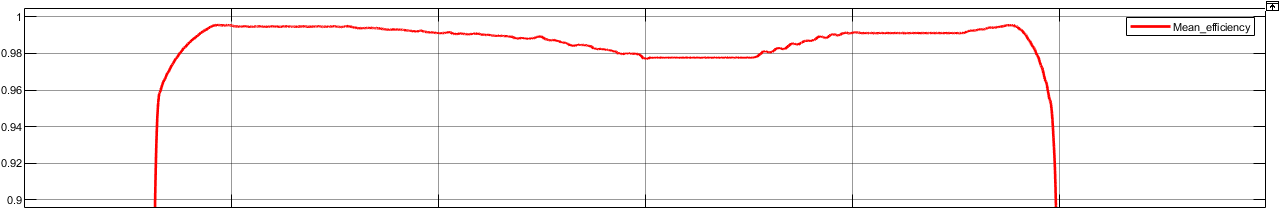
\includegraphics[width=0.5\textwidth]{eficiencia.png}
	\caption{Eficiencia media de la potencia del modelo propuesto}
	\label{eficiencia}
\end{figure}

Finalmente podemos comprobar la eficiencia general del sistema.

\begin{figure}[h!]
	\centering
	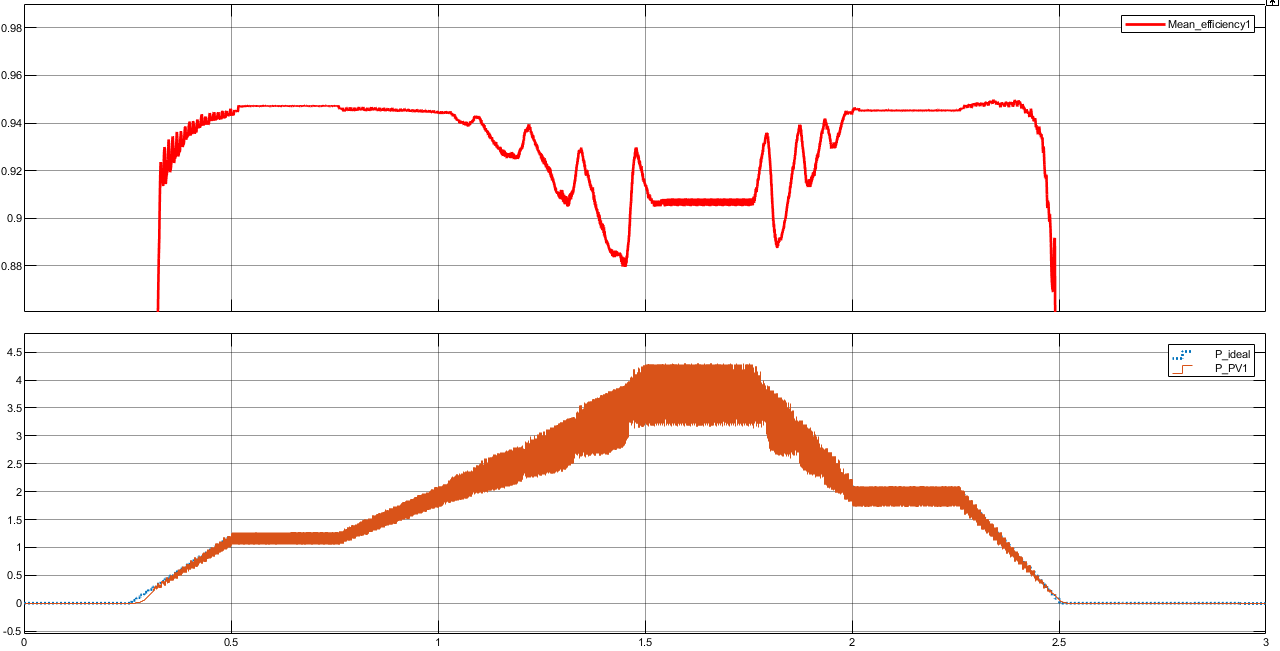
\includegraphics[width=0.5\textwidth]{potencia_curvas_2.png}
	\caption{Eficiencia de la potencia de la carga}
	\label{eficiencia}
\end{figure}

\newpage
\section{Conclusiones}

El algoritmo implementado para el MPPT en el convertidor boost presenta una respuesta satisfactoria ya que la eficiencia del modelo es aproximadamente es del 96 $\%$, lo que fundamenta la importancia del uso de algoritmos para aprovechar la máxima potencia entregada por el sistema fotovoltaico y que pueda mitigar el problema de la no linealidad del modelo matemático que rige este sistema.
Se recomienda proceder con el desarrollo experimental que pueda corroborar dichos resultados. Así mismo simular este sistema con otros algoritmos MPPT para verificar el más apropiado. Finalmente se recomienda variar el ciclo útil en lazo abierto para verificar que la potencia entregada sea la máxima requerida.
\newpage

\bibliographystyle{ieeetr}
\bibliography{mybib}

\end{document}